\documentclass{beamer}
\usefonttheme{serif}

\mode<presentation> {

\usetheme{Frankfurt}

%\setbeamertemplate{footline} % To remove the footer line in all slides uncomment this line
%\setbeamertemplate{footline}[page number] % To replace the footer line in all slides with a simple slide count uncomment this line

%\setbeamertemplate{navigation symbols}{} % To remove the navigation symbols from the bottom of all slides uncomment this line
}

\usepackage{tikz-cd}
\usetikzlibrary{positioning, calc}
\usetikzlibrary{matrix,arrows,decorations.pathmorphing}
\usepackage{mathtools, amsfonts}

\DeclareMathOperator{\coker}{coker}
\DeclareMathOperator{\Hom}{Hom}

\usepackage{graphicx, animate} % Allows including images and animation
%\graphicspath{ {} }

\setbeamertemplate{headline}{}
%----------------------------------------------------------------------------------------
%	TITLE PAGE
%----------------------------------------------------------------------------------------

\title[TDA]{Topology and Data Analysis} % The short title appears at the bottom of every slide, the full title is only on the title page

\author{Dr. Matthew Zabka} % Your name
\institute[SMSU] % Your institution as it will appear on the bottom of every slide, may be shorthand to save space
{
Southwest Minnesota State University \\ % Your institution for the title page
}
\date{26 October 2016} % Date, can be changed to a custom date

%-----------------------------------------------------------------------------------------

\begin{document}
\bibliographystyle{amsalpha}
%-----------------------------------------------------------
\begin{frame}
\titlepage % Print the title page as the first slide
\end{frame}
%----------------------------------------------------------
\begin{frame}
\frametitle{Overview} % Table of contents slide, comment this block out to remove it
\tableofcontents % Throughout your presentation, if you choose to use \section{} and \subsection{} commands, these will automatically be printed on this slide as an overview of your presentation
\end{frame}

%----------------------------------------------------------------------------------------
%	PRESENTATION SLIDES
%----------------------------------------------------------------------------------------
%------------------------------------------------
\section{Topology} 

\begin{frame}
\frametitle{Topology}
\begin{itemize}
\item<1-> One idea in topology is to generalize the idea of continuity that you learn in your calculus class.
\item<2-> We should like to investigate a space's properties that are preserved under continuous deformation.
\item<3-> It is often said the a topologist cannot tell the difference between a coffee cup and a doughnut.
\end{itemize}
\end{frame}


\begin{frame}
\frametitle{Topology}
\begin{center}
\animategraphics[autoplay, loop, scale = 0.75]{4}{/CupToDoughnut/mug}{01}{58}
\end{center}
\end{frame}

\begin{frame}
\frametitle{Topology}
\begin{itemize}
\item<1-> Topologists regard two spaces as `the same' (\textbf{homeomorphic}) whenever one space can be continuously deformed to look like the other space.
\item<2-> No `ripping' and no `gluing'.
\item<3-> In the previous example, the coffee cup and doughnut look the same to a topologist.
\item<4-> What other spaces look the same to a topologist?
\end{itemize}
\end{frame}

\begin{frame}
\frametitle{Topology}
Which of the following do topologists regard as `the same'?

\bigskip

\center{\fontsize{70}{80}\selectfont \textsf{A B C D}}

\end{frame}

\begin{frame}
\frametitle{Topology}
Which of the following do topologists regard as 'the same'?
\bigskip
\center{\fontsize{70}{80}\selectfont \textsf{ {\color{red} A} B C {\color{red} {D}}}}

\end{frame}

\begin{frame}
\frametitle{Topology}
How do we know that these are `the same'?

\center{\fontsize{70}{80}\selectfont \textsf{  A  D }}
\end{frame}

\begin{frame}
\frametitle{Topology}
Because we can find the deformation!
\frametitle{Topology}
\begin{center}
\animategraphics[autoplay, scale = 0.35]{2}{/AtoD/A}{1}{17}
\end{center}
\end{frame}



\begin{frame}
\frametitle{Topology}
\begin{itemize}
\item<1-> How do we know that the following are `different'?
\end{itemize}
\center{\fontsize{70}{80}\selectfont \textsf{  A  B }}
\begin{itemize}
\item<2-> Just because we cannot find a deformation does not mean such a deformation does not exist!
\item<3-> We need more tools in order to prove that two spaces are `different'.
\item<4-> This is why algebraic topology was invented.
\end{itemize}
\end{frame}
%-------------------------------------------------------
\section{Algebraic Topolgy}
\begin{frame}
\frametitle{Algebraic Topology}
\begin{itemize}
\item<1-> We need a way show that no deformation exists between two spaces.
\item<2-> This is a very difficult problem.
\item<3-> We need a workaround.
\end{itemize}
\end{frame}

\begin{frame}
\frametitle{Algebraic Topology}
\begin{itemize}
\item<1-> Abstract Algebra is the study of different {\color{red}algebraic structures}.
	\begin{itemize}
	\item<2-> $\mathbb{R}$
	\item<2-> $\mathbb{Q}$
	\item<2-> $\mathbb{Z}$
	\item<2-> $\mathbb{Z}/p$
	\end{itemize}
\item<3-> Trick: Assign to each topological space algebraic structures in a clever way. 
\item<4-> If two spaces have different structures, then they are not `the same'.
\end{itemize}
\end{frame}


\begin{frame}
\frametitle{Algebraic Topology}
\begin{itemize}
\item<1-> One of the most popular ways to assign an algebraic structure to a topological space $X$ is \textbf{homology}.
\item<2-> The $n$-th homology group, denoted $H_n(X; \mathbb{Z})$, is a very useful algebraic structure.
\item<3-> The $n$-th \textbf{Betti number} $\beta_n$ counts the number of $n$-dimensional holes in a space.
\item<4-> The $n$-th \textbf{Betti number} $\beta_n$ counts the number of $\mathbb{Z}$-summands in $H_n(X;\mathbb{Z})$.
\end{itemize}
\end{frame}

\begin{frame}
\frametitle{Algebraic Topology}
\[ \beta_j = \begin{cases} 
      	1 & j = 0, 1 \\
      	0 & j \neq 1 
   \end{cases}
\]
%\begin{center}
%
\includegraphics[scale=0.3]{S1}
%\end{center}
\end{frame}

\begin{frame}
\frametitle{Algebraic Topology}
\[ \beta_j = \begin{cases} 
      1 & j = 0, 2 \\
      0 & j \neq 2 
   \end{cases}
\]
%\begin{center}
%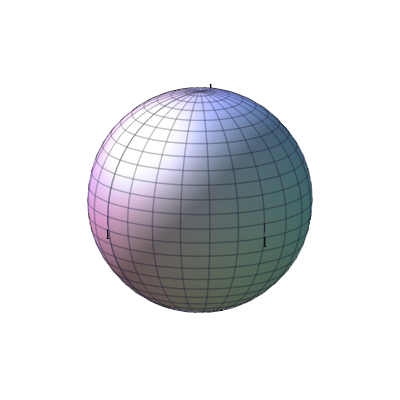
\includegraphics[scale=0.5]{S2}
%\end{center}
\end{frame}

\begin{frame}
\frametitle{Algebraic Topology}
\[ \beta_j = \begin{cases} 
      2 & j = 0, 1 \\
      0 & j \neq 2 
   \end{cases}
\]
%\begin{center}
%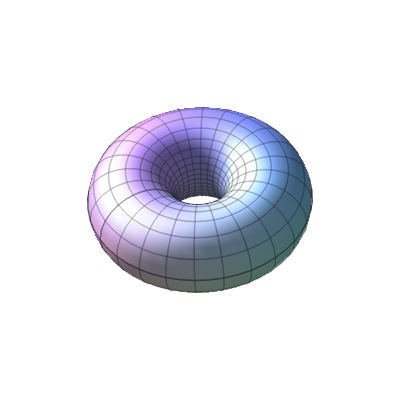
\includegraphics[scale=0.5]{Torus}
%\end{center}
\end{frame}

\begin{frame}
\frametitle{Algebraic Topology}
\begin{itemize}
\item<1-> {\fontsize{70}{80}\selectfont \textsf{  A  }} $\beta_1 = 1$
\item<2-> {\fontsize{70}{80}\selectfont \textsf{  B  }} $\beta_1 = 2$

So A and B are not the same in the eyes of a topologist.
\end{itemize}

\end{frame}
%-------------------------------------------------------
\section{Topological Data Analysis}

\begin{frame}
\frametitle{Topological Data Analysis}
\begin{itemize}
	\item<1-> Big data are a big deal.
	\item<2-> Data often have shape.
	\item<3-> We can use the tools of topology to understand data's shape.
\end{itemize}
\end{frame}

%------------------------------------------------
\begin{frame}
\frametitle{Clustering}
Topological Data Analysis has its roots in a statistical method called \textbf{cluster analysis}. Our goal is to partition the data into subsets called \textbf{clusters}, so that the points in the clusters are ``close'' to each other, but far from points in other clusters. 
\begin{itemize}
	\item<1-> Begin with a set of $n$ points $X_n$.
	\item<2-> Set the parameter $r=0$. Start with each singleton $\{x\}$ of $X$ as its own cluster.
	\item<3-> Increase $r$. For $x$ and $y$ in $X$, merge the clusters containing $x$ and $y$ whenever
	\[
	d(x,y) <r/2.
	\]
	\item<5-> Stop when you have only one cluster.
\end{itemize}
\end{frame}
%-----------------------------------------------
\begin{frame}
\frametitle{Clustering}
\begin{center}
\begin{tikzpicture}
\draw 	(-4.5,4) node[circle,fill,inner sep=1pt](a1){}   (-4,2.5) node[circle,fill,inner sep=1pt](a2){} 
  		(-4.3,4.2) node[circle,fill,inner sep=1pt](a3){};
%\path[-]
%    (a1) edge node {} (a2)
%    (a2) edge node {} (a3)
%    (a3) edge node {} (a1);
    
\draw 	(0.866, 0.5) node[circle,fill,inner sep=1pt](b1){}  (0,1) node[circle,fill,inner sep=1pt](b2){}  
		(-0.866,0.5) node[circle,fill,inner sep=1pt](b3){}  (-0.866,-0.5) node[circle,fill,inner sep=1pt](b4){}
		(0,-1	   ) node[circle,fill,inner sep=1pt](b5){}  (0.866, -0.5) node[circle,fill,inner sep=1pt](b6){};
%\path[-]
%    (b1) edge node {} (b2)
%    (b2) edge node {} (b3)
%    (b3) edge node {} (b4)
%    (b4) edge node {} (b5)
%    (b5) edge node {} (b6)
%    (b6) edge node {} (b1);
\end{tikzpicture}
\end{center}
$r=0$, \quad nine clusters
\end{frame}
%------------------------------------------------
\begin{frame}
\frametitle{Clustering}
\begin{center}
\begin{tikzpicture}
\draw 	(-4.5,4) node[circle,fill,inner sep=1pt](a1){}   (-4,2.5) node[circle,fill,inner sep=1pt](a2){} 
  		(-4.3,4.2) node[circle,fill,inner sep=1pt](a3){};
\path[-]
%    (a1) edge node {} (a2)
%    (a2) edge node {} (a3)
     (a3) edge[red] node {} (a1);
    
\draw 	(0.866, 0.5) node[circle,fill,inner sep=1pt](b1){}  (0,1) node[circle,fill,inner sep=1pt](b2){}  
		(-0.866,0.5) node[circle,fill,inner sep=1pt](b3){}  (-0.866,-0.5) node[circle,fill,inner sep=1pt](b4){}
		(0,-1	   ) node[circle,fill,inner sep=1pt](b5){}  (0.866, -0.5) node[circle,fill,inner sep=1pt](b6){};
%\path[-]
%    (b1) edge node {} (b2)
%    (b2) edge node {} (b3)
%    (b3) edge node {} (b4)
%    (b4) edge node {} (b5)
%    (b5) edge node {} (b6)
%    (b6) edge node {} (b1);
\draw (a1) circle (0.2cm);
\draw (a2) circle (0.2cm);
\draw (a3) circle (0.2cm);
\draw (b1) circle (0.2cm);
\draw (b2) circle (0.2cm);
\draw (b3) circle (0.2cm);
\draw (b4) circle (0.2cm);
\draw (b5) circle (0.2cm);
\draw (b6) circle (0.2cm);
\end{tikzpicture}
\end{center}
$r=0.2$ \quad eight clusters
\end{frame}
%------------------------------------------------
\begin{frame}
\frametitle{Clustering}
\begin{center}
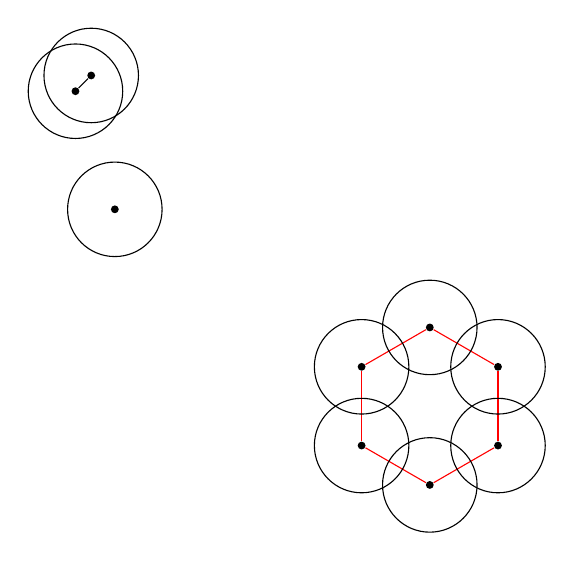
\begin{tikzpicture}
\draw 	(-4.5,4) node[circle,fill,inner sep=1pt](a1){}   (-4,2.5) node[circle,fill,inner sep=1pt](a2){} 
  		(-4.3,4.2) node[circle,fill,inner sep=1pt](a3){};
\path[-]
%    (a1) edge node {} (a2)
%    (a2) edge node {} (a3)
     (a3) edge node {} (a1);
    
\draw 	(0.866, 0.5) node[circle,fill,inner sep=1pt](b1){}  (0,1) node[circle,fill,inner sep=1pt](b2){}  
		(-0.866,0.5) node[circle,fill,inner sep=1pt](b3){}  (-0.866,-0.5) node[circle,fill,inner sep=1pt](b4){}
		(0,-1	   ) node[circle,fill,inner sep=1pt](b5){}  (0.866, -0.5) node[circle,fill,inner sep=1pt](b6){};
\path[-]
    (b1) edge[red] node {} (b2)
    (b2) edge[red] node {} (b3)
    (b3) edge[red] node {} (b4)
    (b4) edge[red] node {} (b5)
    (b5) edge[red] node {} (b6)
    (b6) edge[red] node {} (b1);
\draw (a1) circle (0.6cm);
\draw (a2) circle (0.6cm);
\draw (a3) circle (0.6cm);
\draw (b1) circle (0.6cm);
\draw (b2) circle (0.6cm);
\draw (b3) circle (0.6cm);
\draw (b4) circle (0.6cm);
\draw (b5) circle (0.6cm);
\draw (b6) circle (0.6cm);
\end{tikzpicture}
\end{center}
$r=0.6$ \quad three clusters
\end{frame}
%------------------------------------------------
\begin{frame}
\frametitle{Clustering}
\begin{center}
\begin{tikzpicture}
\draw 	(-4.5,4) node[circle,fill,inner sep=1pt](a1){}   (-4,2.5) node[circle,fill,inner sep=1pt](a2){} 
  		(-4.3,4.2) node[circle,fill,inner sep=1pt](a3){};
\path[-]
     (a1) edge[red] node {} (a2)
%    (a2) edge node {} (a3)
     (a3) edge node {} (a1);
    
\draw 	(0.866, 0.5) node[circle,fill,inner sep=1pt](b1){}  (0,1) node[circle,fill,inner sep=1pt](b2){}  
		(-0.866,0.5) node[circle,fill,inner sep=1pt](b3){}  (-0.866,-0.5) node[circle,fill,inner sep=1pt](b4){}
		(0,-1	   ) node[circle,fill,inner sep=1pt](b5){}  (0.866, -0.5) node[circle,fill,inner sep=1pt](b6){};
\path[-]
    (b1) edge node {} (b2)
    (b2) edge node {} (b3)
    (b3) edge node {} (b4)
    (b4) edge node {} (b5)
    (b5) edge node {} (b6)
    (b6) edge node {} (b1);
\draw (a1) circle (0.8cm);
\draw (a2) circle (0.8cm);
\draw (a3) circle (0.8cm);
%\draw (b1) circle (0.8cm);
%\draw (b2) circle (0.8cm);
\draw (b3) circle (0.8cm);
%\draw (b4) circle (0.8cm);
%\draw (b5) circle (0.8cm);
%\draw (b6) circle (0.8cm);
\end{tikzpicture}
\end{center}
$r=0.8$ \quad two clusters
\end{frame}
%------------------------------------------------
\begin{frame}
\frametitle{Clustering}
\begin{center}
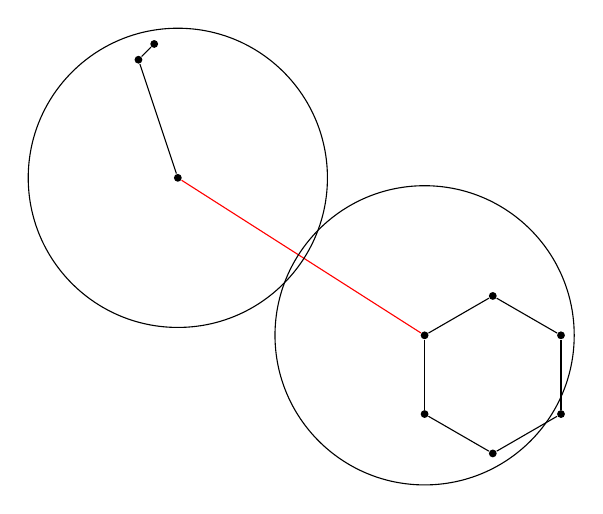
\begin{tikzpicture}
\draw 	(-4.5,4) node[circle,fill,inner sep=1pt](a1){}   (-4,2.5) node[circle,fill,inner sep=1pt](a2){} 
  		(-4.3,4.2) node[circle,fill,inner sep=1pt](a3){};
\path[-]
     (a1) edge node {} (a2)
%    (a2) edge node {} (a3)
     (a3) edge node {} (a1);
    
\draw 	(0.866, 0.5) node[circle,fill,inner sep=1pt](b1){}  (0,1) node[circle,fill,inner sep=1pt](b2){}  
		(-0.866,0.5) node[circle,fill,inner sep=1pt](b3){}  (-0.866,-0.5) node[circle,fill,inner sep=1pt](b4){}
		(0,-1	   ) node[circle,fill,inner sep=1pt](b5){}  (0.866, -0.5) node[circle,fill,inner sep=1pt](b6){};
\path[-]
    (b1) edge node {} (b2)
    (b2) edge node {} (b3)
    (b3) edge node {} (b4)
    (b4) edge node {} (b5)
    (b5) edge node {} (b6)
    (b6) edge node {} (b1)
    (a2) edge[red] node {} (b3);
%\draw (a1) circle (0.8cm);
\draw (a2) circle (1.9cm);
%\draw (a3) circle (0.8cm);
%\draw (b1) circle (0.8cm);
%\draw (b2) circle (0.8cm);
\draw (b3) circle (1.9cm);
%\draw (b4) circle (0.8cm);
%\draw (b5) circle (0.8cm);
%\draw (b6) circle (0.8cm);
\end{tikzpicture}
\end{center}
$r=1.9$ \quad one cluster
\end{frame}
%------------------------------------------------
\begin{frame}
\frametitle{Clustering}
\begin{center}
\begin{tikzpicture}[scale = 0.9]
\draw 	(-4.5,4) node[circle,fill,inner sep=1pt](a1){}   (-4,2.5) node[circle,fill,inner sep=1pt](a2){} 
  		(-4.3,4.2) node[circle,fill,inner sep=1pt](a3){};
\path[-]
     (a1) edge node {} (a2)
%    (a2) edge node {} (a3)
     (a3) edge node {} (a1);
    
\draw 	(0.866, 0.5) node[circle,fill,inner sep=1pt](b1){}  (0,1) node[circle,fill,inner sep=1pt](b2){}  
		(-0.866,0.5) node[circle,fill,inner sep=1pt](b3){}  (-0.866,-0.5) node[circle,fill,inner sep=1pt](b4){}
		(0,-1	   ) node[circle,fill,inner sep=1pt](b5){}  (0.866, -0.5) node[circle,fill,inner sep=1pt](b6){};
\path[-]
    (b1) edge node {} (b2)
    (b2) edge node {} (b3)
    (b3) edge node {} (b4)
    (b4) edge node {} (b5)
    (b5) edge node {} (b6)
    (b6) edge node {} (b1);
%   (a2) edge node {} (b3)
\end{tikzpicture}
\end{center}
\begin{itemize}
	\item<1-> For any $r>0$, we have partitioned the data into clusters.
	\item<2-> Which $r$ is correct? (Gives information about the data)
	\item<3-> GOAL: Find which clusters \textit{persist} over a large range of $r$.
	\item<4-> Conclude that these clusters are genuine to the data's structure.
\end{itemize}
\end{frame}
%-----------------------------------------------------------------
\begin{frame}
\frametitle{Clustering}
A \textit{dendogram} can help us see which clusters persist over a large range of $r$ -- called \textit{height} on the $y$-axis in the dendogram below.
\begin{figure}
%\begin{center}
%	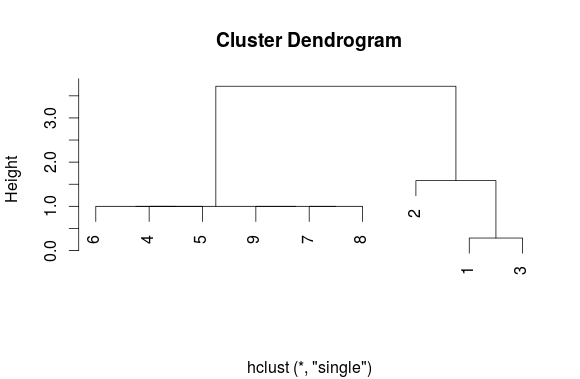
\includegraphics[width=70mm]{SimpleDen}
%	\caption{Dendogram of single linkage clustering for above data set}
%\end{center}
\end{figure}
\end{frame}
%----------------------------------------------------------------
\begin{frame}
\frametitle{Topological Data Analysis}
\begin{center}
\begin{tikzpicture}
\draw 	(-4.5,4) node[circle,fill,inner sep=1pt](a1){}   (-4,2.5) node[circle,fill,inner sep=1pt](a2){} 
  		(-4.3,4.2) node[circle,fill,inner sep=1pt](a3){};
\path[-]
     (a1) edge node {} (a2)
%    (a2) edge node {} (a3)
     (a3) edge node {} (a1);
    
\draw 	(0.866, 0.5) node[circle,fill,inner sep=1pt](b1){}  (0,1) node[circle,fill,inner sep=1pt](b2){}  
		(-0.866,0.5) node[circle,fill,inner sep=1pt](b3){}  (-0.866,-0.5) node[circle,fill,inner sep=1pt](b4){}
		(0,-1	   ) node[circle,fill,inner sep=1pt](b5){}  (0.866, -0.5) node[circle,fill,inner sep=1pt](b6){};
\path[-]
    (b1) edge node {} (b2)
    (b2) edge node {} (b3)
    (b3) edge node {} (b4)
    (b4) edge node {} (b5)
    (b5) edge node {} (b6)
    (b6) edge node {} (b1);
%   (a2) edge node {} (b3)
\end{tikzpicture}
\end{center}
\begin{itemize}
\item<1-> We have created a topological space. The \textit{clusters} are \textit{connected components}.
\item<2-> How can we generalize this process to find higher structure in the data?
\end{itemize}
\end{frame}
%----------------------------------------------------------------------
\begin{frame}
\frametitle{Topological Data Analysis}
GOAL: Create a topological space from data
\begin{itemize}
\item<1-> As before, start with a data set $X_n$ with $n$ points in a metric space with metric $d$.
\item<2-> Set $r=0$. Start with the discrete topology on $X_n$.
\item<3-> Increase $r$. 
	\begin{itemize}
	\item For $x_0$ and $x_1$ in $X_n$, let an edge exist between $x_0$ and $x_1$ if and only if $d(x_0,x_1)<r$.
	\item More generally, for $x_0, x_1, \ldots, x_k$, let a $k$-simplex exist between these points if and only if $d(x_i,x_j)<r$ for all $i, j$. (Vietoris-Rips Complex)
	\item Note: The topological space we create is a simplicial complex.
	\end{itemize}
\item<4-> The topological structure that persists over a large range of $r$ gives us information about the genuine structure of the data.
\item<5-> In particular, we should like to know which generators of homology groups persist over time.
\end{itemize}
\end{frame}
%-------------------------------------------------------------------
\begin{frame}
\frametitle{Topological Data Analysis}
\begin{center}
\begin{tikzpicture}
\draw 	(-4.5,4) node[circle,fill,inner sep=1pt](a1){}   (-4,2.5) node[circle,fill,inner sep=1pt](a2){} 
  		(-4.3,4.2) node[circle,fill,inner sep=1pt](a3){};
    
\draw 	(0.866, 0.5) node[circle,fill,inner sep=1pt](b1){}  (0,1) node[circle,fill,inner sep=1pt](b2){}  
		(-0.866,0.5) node[circle,fill,inner sep=1pt](b3){}  (-0.866,-0.5) node[circle,fill,inner sep=1pt](b4){}
		(0,-1	   ) node[circle,fill,inner sep=1pt](b5){}  (0.866, -0.5) node[circle,fill,inner sep=1pt](b6){};
\end{tikzpicture}
\end{center}
$r=0$
\end{frame}
%--------------------------------------------
\begin{frame}
\frametitle{Topological Data Analysis}
\begin{center}
\begin{tikzpicture}
\draw 	(-4.5,4) node[circle,fill,inner sep=1pt](a1){}   (-4,2.5) node[circle,fill,inner sep=1pt](a2){} 
  		(-4.3,4.2) node[circle,fill,inner sep=1pt](a3){};
\path[-]
%     (a1) edge node {} (a2)
%     (a2) edge node {} (a3)
      (a3) edge[red] node {} (a1);
    
\draw 	(0.866, 0.5) node[circle,fill,inner sep=1pt](b1){}  (0,1) node[circle,fill,inner sep=1pt](b2){}  
		(-0.866,0.5) node[circle,fill,inner sep=1pt](b3){}  (-0.866,-0.5) node[circle,fill,inner sep=1pt](b4){}
		(0,-1	   ) node[circle,fill,inner sep=1pt](b5){}  (0.866, -0.5) node[circle,fill,inner sep=1pt](b6){};
%\path[-]
%    (b1) edge node {} (b2)
%    (b2) edge node {} (b3)
%    (b3) edge node {} (b4)
%    (b4) edge node {} (b5)
%    (b5) edge node {} (b6)
%    (b6) edge node {} (b1)
%    (a2) edge node {} (b3);
\draw (a1) circle (0.2cm);
\draw (a2) circle (0.2cm);
\draw (a3) circle (0.2cm);
\draw (b1) circle (0.2cm);
\draw (b2) circle (0.2cm);
\draw (b3) circle (0.2cm);
\draw (b4) circle (0.2cm);
\draw (b5) circle (0.2cm);
\draw (b6) circle (0.2cm);
\end{tikzpicture}
\end{center}
$r=0.2$
\end{frame}
%-------------------------------------------------------------------
\begin{frame}
\frametitle{Clustering}
\begin{center}
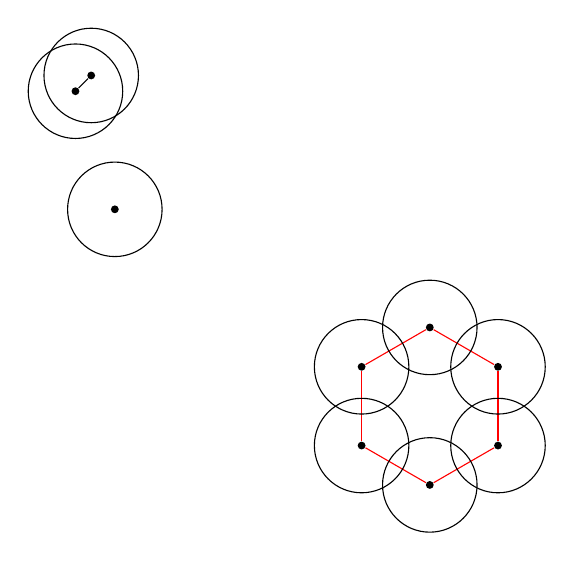
\begin{tikzpicture}
\draw 	(-4.5,4) node[circle,fill,inner sep=1pt](a1){}   (-4,2.5) node[circle,fill,inner sep=1pt](a2){} 
  		(-4.3,4.2) node[circle,fill,inner sep=1pt](a3){};
\path[-]
%    (a1) edge node {} (a2)
%    (a2) edge node {} (a3)
     (a3) edge node {} (a1);
    
\draw 	(0.866, 0.5) node[circle,fill,inner sep=1pt](b1){}  (0,1) node[circle,fill,inner sep=1pt](b2){}  
		(-0.866,0.5) node[circle,fill,inner sep=1pt](b3){}  (-0.866,-0.5) node[circle,fill,inner sep=1pt](b4){}
		(0,-1	   ) node[circle,fill,inner sep=1pt](b5){}  (0.866, -0.5) node[circle,fill,inner sep=1pt](b6){};
\path[-]
    (b1) edge[red] node {} (b2)
    (b2) edge[red] node {} (b3)
    (b3) edge[red] node {} (b4)
    (b4) edge[red] node {} (b5)
    (b5) edge[red] node {} (b6)
    (b6) edge[red] node {} (b1);
\draw (a1) circle (0.6cm);
\draw (a2) circle (0.6cm);
\draw (a3) circle (0.6cm);
\draw (b1) circle (0.6cm);
\draw (b2) circle (0.6cm);
\draw (b3) circle (0.6cm);
\draw (b4) circle (0.6cm);
\draw (b5) circle (0.6cm);
\draw (b6) circle (0.6cm);
\end{tikzpicture}
\end{center}
$r=0.6$, $\beta_1 = 1$
\end{frame}
%------------------------------------------------
\begin{frame}
\frametitle{Clustering}
\begin{center}
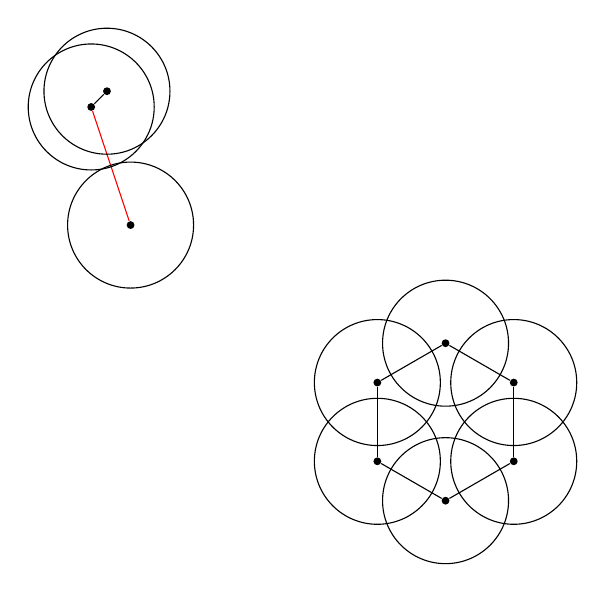
\begin{tikzpicture}
\draw 	(-4.5,4) node[circle,fill,inner sep=1pt](a1){}   (-4,2.5) node[circle,fill,inner sep=1pt](a2){} 
  		(-4.3,4.2) node[circle,fill,inner sep=1pt](a3){};
\path[-]
     (a1) edge[red] node {} (a2)
%    (a2) edge node {} (a3)
     (a3) edge node {} (a1);
    
\draw 	(0.866, 0.5) node[circle,fill,inner sep=1pt](b1){}  (0,1) node[circle,fill,inner sep=1pt](b2){}  
		(-0.866,0.5) node[circle,fill,inner sep=1pt](b3){}  (-0.866,-0.5) node[circle,fill,inner sep=1pt](b4){}
		(0,-1	   ) node[circle,fill,inner sep=1pt](b5){}  (0.866, -0.5) node[circle,fill,inner sep=1pt](b6){};
\path[-]
    (b1) edge node {} (b2)
    (b2) edge node {} (b3)
    (b3) edge node {} (b4)
    (b4) edge node {} (b5)
    (b5) edge node {} (b6)
    (b6) edge node {} (b1);
\draw (a1) circle (0.8cm);
\draw (a2) circle (0.8cm);
\draw (a3) circle (0.8cm);
\draw (b1) circle (0.8cm);
\draw (b2) circle (0.8cm);
\draw (b3) circle (0.8cm);
\draw (b4) circle (0.8cm);
\draw (b5) circle (0.8cm);
\draw (b6) circle (0.8cm);
\end{tikzpicture}
\end{center}
$r=0.8$ 
\end{frame}
%------------------------------------------------
\begin{frame}
\frametitle{Clustering}
\begin{center}
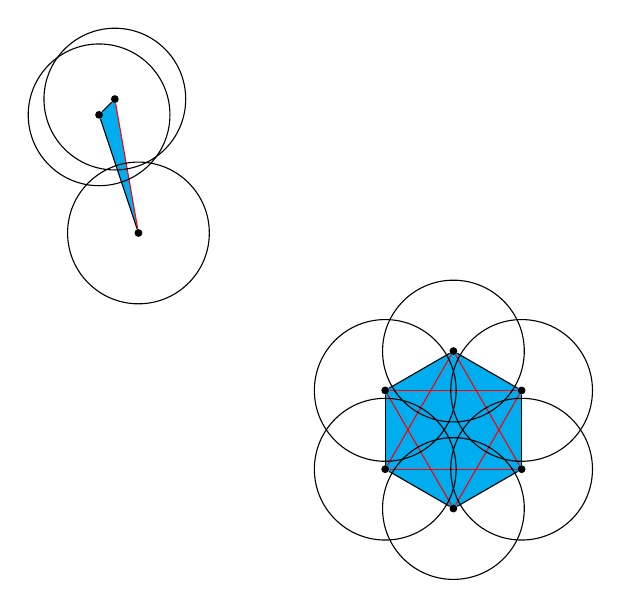
\begin{tikzpicture}
\path [blue, fill=cyan, thick] (-4.5,4) 	-- (-4, 2.5) 	-- (-4.3, 4.2);
\path [blue, fill=cyan, thick] (0.866, 0.5) -- (0,1) 		-- (-0.866,0.5);
\path [blue, fill=cyan, thick] (0,1) 		-- (-0.866,0.5) -- (-0.866,-0.5);
\path [blue, fill=cyan, thick] (-0.866,0.5) -- (-0.866,-0.5)-- (0,-1);
\path [blue, fill=cyan, thick] (-0.866,-0.5)-- (0,-1)		-- (0.866, -0.5);
\path [blue, fill=cyan, thick] (0,-1)		-- (0.866, -0.5)-- (0.866, 0.5);
\path [blue, fill=cyan, thick] (0.866, -0.5)-- (0.866, 0.5) -- (0,1);
\path [blue, fill=cyan, thick] (-0.866,-0.5) -- (0, 1) 		-- (0.866, -0.5);

\draw 	(-4.5,4) node[circle,fill,inner sep=1pt](a1){}   (-4,2.5) node[circle,fill,inner sep=1pt](a2){} 
  		(-4.3,4.2) node[circle,fill,inner sep=1pt](a3){};
\path[-]
     (a1) edge node {} (a2)
     (a2) edge[red] node {} (a3)
     (a3) edge node {} (a1);
    
\draw 	(0.866, 0.5) node[circle,fill,inner sep=1pt](b1){}  (0,1) node[circle,fill,inner sep=1pt](b2){}  
		(-0.866,0.5) node[circle,fill,inner sep=1pt](b3){}  (-0.866,-0.5) node[circle,fill,inner sep=1pt](b4){}
		(0,-1	   ) node[circle,fill,inner sep=1pt](b5){}  (0.866, -0.5) node[circle,fill,inner sep=1pt](b6){};
\path[-]
    (b1) edge node {} (b2)
    (b2) edge node {} (b3)
    (b3) edge node {} (b4)
    (b4) edge node {} (b5)
    (b5) edge node {} (b6)
    (b6) edge node {} (b1)
    (b1) edge[red] node {} (b3)
    (b2) edge[red] node {} (b4)
    (b3) edge[red] node {} (b5)
    (b4) edge[red] node {} (b6)
    (b5) edge[red] node {} (b1)
    (b6) edge[red] node {} (b2);
\draw (a1) circle (0.9cm);
\draw (a2) circle (0.9cm);
\draw (a3) circle (0.9cm);
\draw (b1) circle (0.9cm);
\draw (b2) circle (0.9cm);
\draw (b3) circle (0.9cm);
\draw (b4) circle (0.9cm);
\draw (b5) circle (0.9cm);
\draw (b6) circle (0.9cm);
\end{tikzpicture}
\end{center}
$r=0.9$, $\beta_2=1$
\end{frame}
%------------------------------------------------
\begin{frame}
\frametitle{Topological Data Analysis}
\begin{center}
\begin{figure}
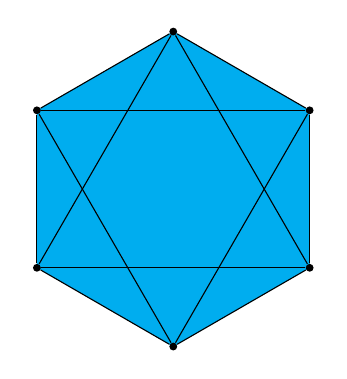
\begin{tikzpicture}[scale = 2]
\path [blue, fill=cyan, thick] (0.866, 0.5) -- (0,1) 		-- (-0.866,0.5);
\path [blue, fill=cyan, thick] (0,1) 		-- (-0.866,0.5) -- (-0.866,-0.5);
\path [blue, fill=cyan, thick] (-0.866,0.5) -- (-0.866,-0.5)-- (0,-1);
\path [blue, fill=cyan, thick] (-0.866,-0.5)-- (0,-1)		-- (0.866, -0.5);
\path [blue, fill=cyan, thick] (0,-1)		-- (0.866, -0.5)-- (0.866, 0.5);
\path [blue, fill=cyan, thick] (0.866, -0.5)-- (0.866, 0.5) -- (0,1);
\path [blue, fill=cyan, thick] (-0.866,-0.5) -- (0, 1) 		-- (0.866, -0.5);
    
\draw 	(0.866, 0.5) node[circle,fill,inner sep=1pt](b1){}  (0,1) node[circle,fill,inner sep=1pt](b2){}  
		(-0.866,0.5) node[circle,fill,inner sep=1pt](b3){}  (-0.866,-0.5) node[circle,fill,inner sep=1pt](b4){}
		(0,-1	   ) node[circle,fill,inner sep=1pt](b5){}  (0.866, -0.5) node[circle,fill,inner sep=1pt](b6){};
\path[-]
    (b1) edge node {} (b2)
    (b2) edge node {} (b3)
    (b3) edge node {} (b4)
    (b4) edge node {} (b5)
    (b5) edge node {} (b6)
    (b6) edge node {} (b1)
    (b1) edge node {} (b3)
    (b2) edge node {} (b4)
    (b3) edge node {} (b5)
    (b4) edge node {} (b6)
    (b5) edge node {} (b1)
    (b6) edge node {} (b2);
\end{tikzpicture}
\caption{$S^2$ as geometrically realized in $\mathbb{R}^2$}
\end{figure}
\end{center}
\end{frame}

%------------------------------------------------
\begin{frame}
\frametitle{Topological Data Analysis}
\begin{center}
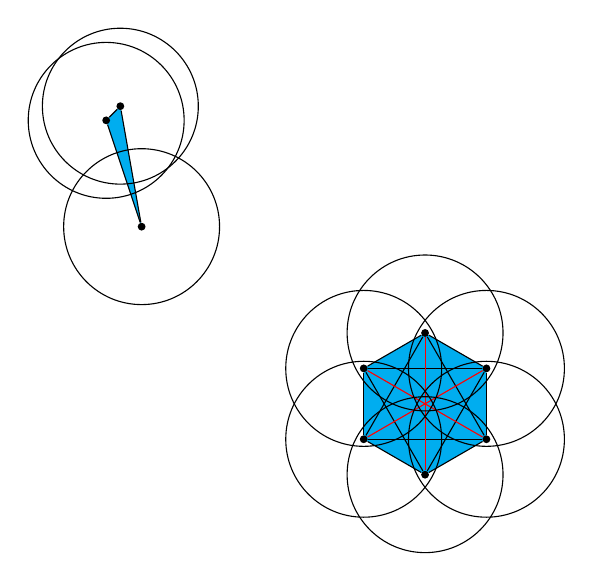
\begin{tikzpicture}[scale = 0.9]
\path [blue, fill=cyan, thick] (-4.5,4) 	-- (-4, 2.5) 	-- (-4.3, 4.2);
\path [blue, fill=cyan, thick] (0.866, 0.5) -- (0,1) 		-- (-0.866,0.5) -- (-0.866,-0.5) -- (0,-1) -- (0.866, -0.5);
\draw 	(-4.5,4) node[circle,fill,inner sep=1pt](a1){}   (-4,2.5) node[circle,fill,inner sep=1pt](a2){} 
  		(-4.3,4.2) node[circle,fill,inner sep=1pt](a3){};
\path[-]
     (a1) edge node {} (a2)
     (a2) edge node {} (a3)
     (a3) edge node {} (a1);
    
\draw 	(0.866, 0.5) node[circle,fill,inner sep=1pt](b1){}  (0,1) node[circle,fill,inner sep=1pt](b2){}  
		(-0.866,0.5) node[circle,fill,inner sep=1pt](b3){}  (-0.866,-0.5) node[circle,fill,inner sep=1pt](b4){}
		(0,-1	   ) node[circle,fill,inner sep=1pt](b5){}  (0.866, -0.5) node[circle,fill,inner sep=1pt](b6){};
\path[-]
    (b1) edge node {} (b2)
    (b2) edge node {} (b3)
    (b3) edge node {} (b4)
    (b4) edge node {} (b5)
    (b5) edge node {} (b6)
    (b6) edge node {} (b1)
    (b1) edge node {} (b3)
    (b2) edge node {} (b4)
    (b3) edge node {} (b5)
    (b4) edge node {} (b6)
    (b5) edge node {} (b1)
    (b6) edge node {} (b2)
    (b1) edge[red] node {} (b4)
    (b2) edge[red] node {} (b5)
    (b3) edge[red] node {} (b6);
    
\draw (a1) circle (1.1cm);
\draw (a2) circle (1.1cm);
\draw (a3) circle (1.1cm);
\draw (b1) circle (1.1cm);
\draw (b2) circle (1.1cm);
\draw (b3) circle (1.1cm);
\draw (b4) circle (1.1cm);
\draw (b5) circle (1.1cm);
\draw (b6) circle (1.1cm);
\end{tikzpicture}
\end{center}
$r=1.1$
\end{frame}

%-----------------------------------------------
\begin{frame}
\frametitle{Topological Data Analysis}
\begin{figure}
\begin{center}
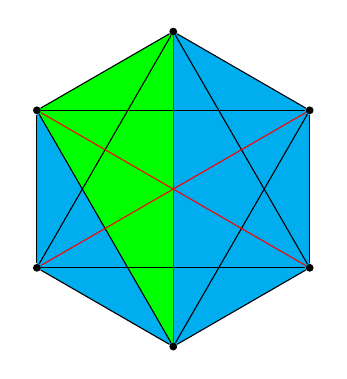
\begin{tikzpicture}[scale = 2]
\path [blue, fill=cyan, thick] (0.866, 0.5) -- (0,1) 		-- (-0.866,0.5) -- (-0.866,-0.5) -- (0,-1) -- (0.866, -0.5);
\path [blue, fill=green, thick] (0,1) 	    -- (-0.866,0.5)	-- (0,-1);
\draw 	(0.866, 0.5) node[circle,fill,inner sep=1pt](b1){}  (0,1) node[circle,fill,inner sep=1pt](b2){}  
		(-0.866,0.5) node[circle,fill,inner sep=1pt](b3){}  (-0.866,-0.5) node[circle,fill,inner sep=1pt](b4){}
		(0,-1	   ) node[circle,fill,inner sep=1pt](b5){}  (0.866, -0.5) node[circle,fill,inner sep=1pt](b6){};
\path[-]
    (b1) edge node {} (b2)
    (b2) edge node {} (b3)
    (b3) edge node {} (b4)
    (b4) edge node {} (b5)
    (b5) edge node {} (b6)
    (b6) edge node {} (b1)
    (b1) edge node {} (b3)
    (b2) edge node {} (b4)
    (b3) edge node {} (b5)
    (b4) edge node {} (b6)
    (b5) edge node {} (b1)
    (b6) edge node {} (b2)
    (b1) edge[red] node {} (b4)
    (b2) edge[red] node {} (b5)
    (b3) edge[red] node {} (b6);
\end{tikzpicture}
\caption{The green triangle is now a $2$-simplex in our space.}
\end{center}
\end{figure}
\end{frame}

%------------------------------------------------
\begin{frame}
\frametitle{Topological Data Analysis}
\begin{center}
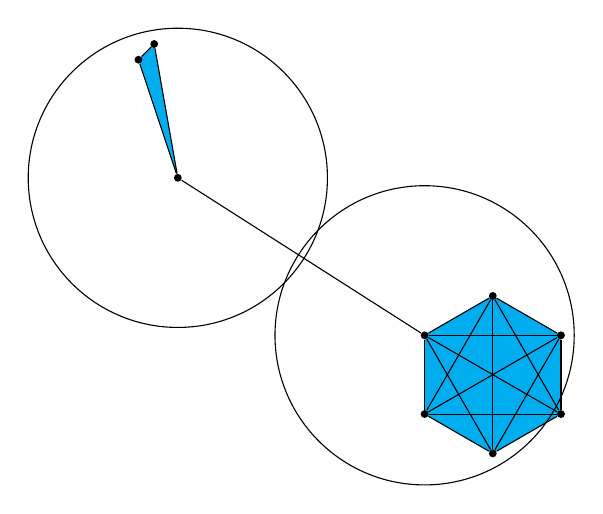
\begin{tikzpicture}
\path [blue, fill=cyan, thick] (-4.5,4) 	-- (-4, 2.5) 	-- (-4.3, 4.2);
\path [blue, fill=cyan, thick] (0.866, 0.5) -- (0,1) 		-- (-0.866,0.5) -- (-0.866,-0.5) -- (0,-1) -- (0.866, -0.5);
\draw 	(-4.5,4) node[circle,fill,inner sep=1pt](a1){}   (-4,2.5) node[circle,fill,inner sep=1pt](a2){} 
  		(-4.3,4.2) node[circle,fill,inner sep=1pt](a3){};
\path[-]
     (a1) edge node {} (a2)
     (a2) edge node {} (a3)
     (a3) edge node {} (a1);
    
\draw 	(0.866, 0.5) node[circle,fill,inner sep=1pt](b1){}  (0,1) node[circle,fill,inner sep=1pt](b2){}  
		(-0.866,0.5) node[circle,fill,inner sep=1pt](b3){}  (-0.866,-0.5) node[circle,fill,inner sep=1pt](b4){}
		(0,-1	   ) node[circle,fill,inner sep=1pt](b5){}  (0.866, -0.5) node[circle,fill,inner sep=1pt](b6){};
\path[-]
    (b1) edge node {} (b2)
    (b2) edge node {} (b3)
    (b3) edge node {} (b4)
    (b4) edge node {} (b5)
    (b5) edge node {} (b6)
    (b6) edge node {} (b1)
    (b1) edge node {} (b3)
    (b2) edge node {} (b4)
    (b3) edge node {} (b5)
    (b4) edge node {} (b6)
    (b5) edge node {} (b1)
    (b6) edge node {} (b2)
    (b1) edge node {} (b4)
    (b2) edge node {} (b5)
    (b3) edge node {} (b6)
    (b3) edge node {} (a2);
    
%\draw (a1) circle (1.1cm);
\draw (a2) circle (1.9cm);
%\draw (a3) circle (1.1cm);
%\draw (b1) circle (1.1cm);
%\draw (b2) circle (1.1cm);
\draw (b3) circle (1.9cm);
%\draw (b4) circle (1.1cm);
%\draw (b5) circle (1.1cm);
%\draw (b6) circle (1.1cm);
\end{tikzpicture}
\end{center}
$r=1.9$
\end{frame}
%-----------------------------------------------
\begin{frame}
\frametitle{Topological Data Analysis}
\begin{itemize}
\item<1-> We're interested in the cases where we can't see the data.
\item<2-> We need a way to see which generators of $H_k$ persist over time.
\item<3-> We can do this with a barcode.
\end{itemize}
\end{frame}


%------------------------------------------------
\begin{frame}
\frametitle{Barcodes}
\begin{figure}
%\begin{center}
%	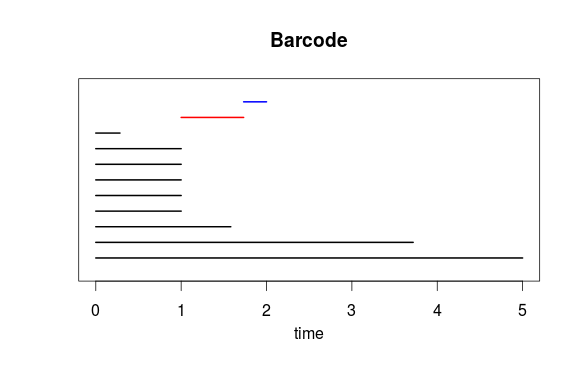
\includegraphics[width=70mm]{SimpleBar}
%	\caption{Barcode for the above data set}
%\end{center}
\end{figure}
\end{frame}

%-----------------------------------------------
\begin{frame}
\frametitle{Barcodes}
Problem: Barcodes can be very messy. In the following, it is difficult to see how many generators for homology exists for a given $r$. Is there another way to  represent this information?
\begin{figure}
%\begin{center}
%	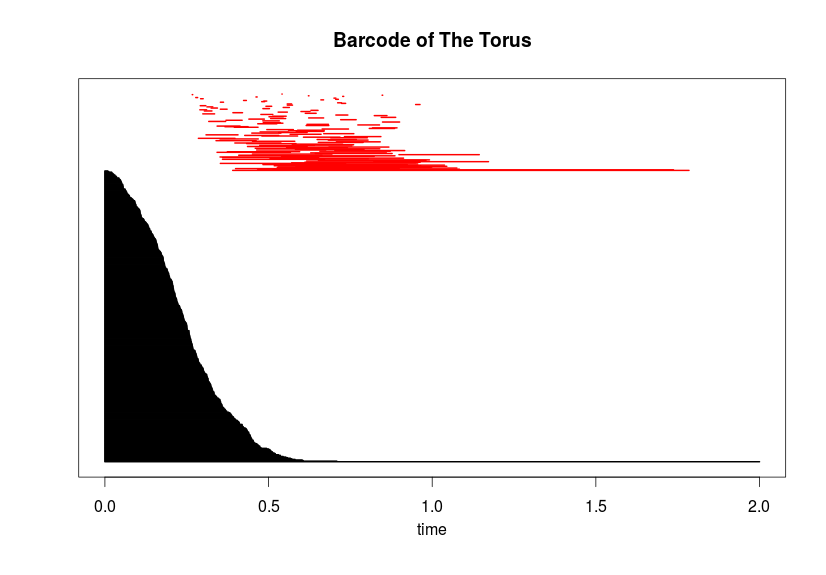
\includegraphics[width=70mm]{TorusBar}
%	\caption{It is hard to see how many generators are in each dimension.}
%\end{center}
\end{figure}
\end{frame}

%-----------------------------------------------
\begin{frame}
\frametitle{Persistence Diagrams}
\begin{itemize}
\item<1-> Each generator has a birth time and a death time.
\item<2-> Plot with the birth time on the $x$-axis and the death time on the $y$-axis and we get a persistence diagram.
\item<3-> It is easier to see the generators that persist over a long period of time.
\end{itemize}
\end{frame}

%---------------------------------------------
\begin{frame}
\frametitle{Persistence Diagrams}
\begin{figure}
%\begin{center}
%	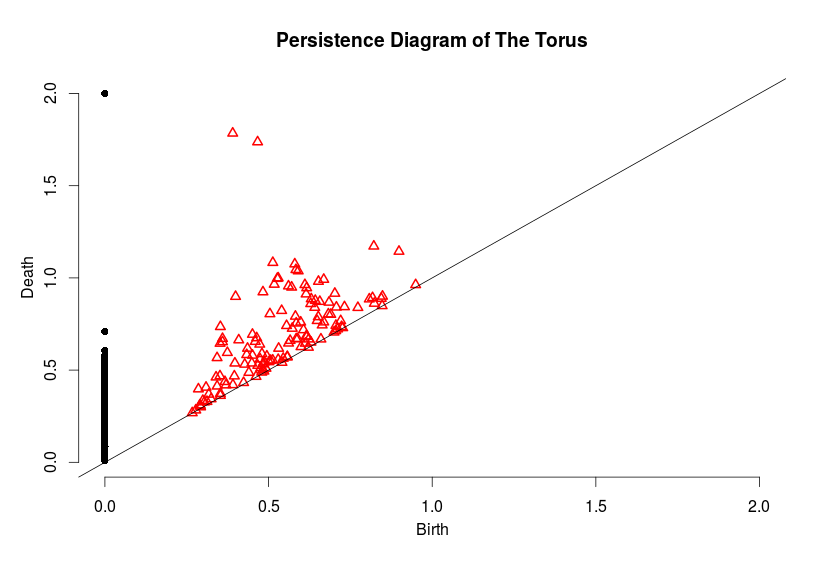
\includegraphics[width=80mm]{TorusPer}
%	\caption{Black circles are generators of $H_0$, Red Triangles are generators of $H_1$}
%\end{center}
\end{figure}
\end{frame}
%---------------------------------------------

\begin{frame}
\frametitle{Why are Asymptotics Important?}
\begin{itemize}
\item<1-> We must decide which generators are genuine to the structure of the data.
\item<2-> \textbf{How far must a generator lie from the line $y=x$ in order to conclude that it represents structure in the data?}
\end{itemize}
\begin{figure}
%\begin{center}
%	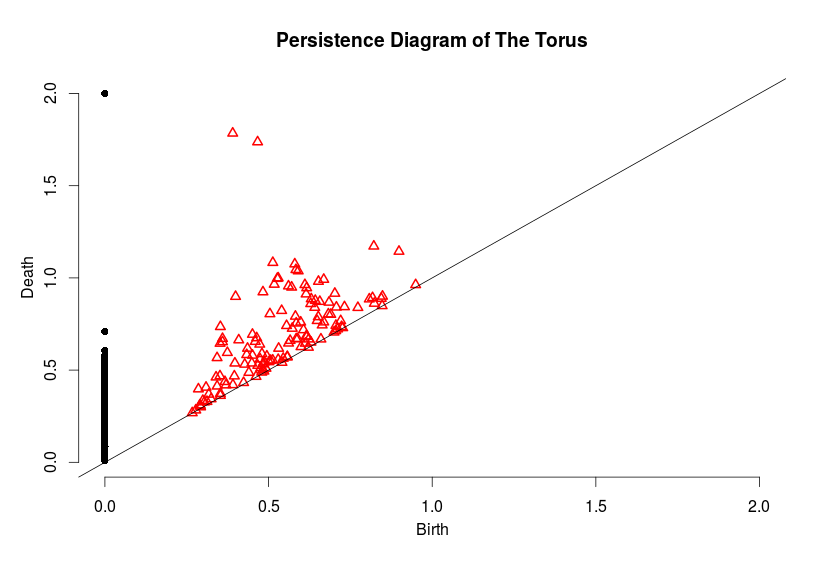
\includegraphics[width=50mm]{TorusPer}
%\end{center}
\end{figure}
\end{frame}
%--------------------------------------------

\begin{frame}
\frametitle{Why are Asymptotics Important?}
\begin{itemize}
\item To answer this question, we must have some underlying probabilistic model.
	\begin{itemize}
	\item[-] Bootstrapping
	\item[-] Study the space of all persistence diagrams
	\item[-] Study the space of all random topological spaces.
	\end{itemize}
\end{itemize}
\end{frame}
%-------------------------------------------------------
\begin{frame}
\frametitle{Thank you!}
\center{\Huge{Questions?}}
\end{frame}
%-------------------------------------------------------
\begin{frame}
\bibliography{Master}
\end{frame}
%-------------------------------------------------------

\end{document} 